\subsection{RIS-aided Dual-Functional Radar and Communications Beamforming Design}

\begin{frame}
    \frametitle{RIS-aided Dual-Functional Radar and Communications Beamforming Design}
    \begin{block}{What}
        \small
        An integrated radar and communication system that can simultaneously track a target and serve multiple communication users.
        A reconfigurable intelligent surface is deployed to improve the system performance.   
    \end{block}
    \begin{figure}
        \centering
        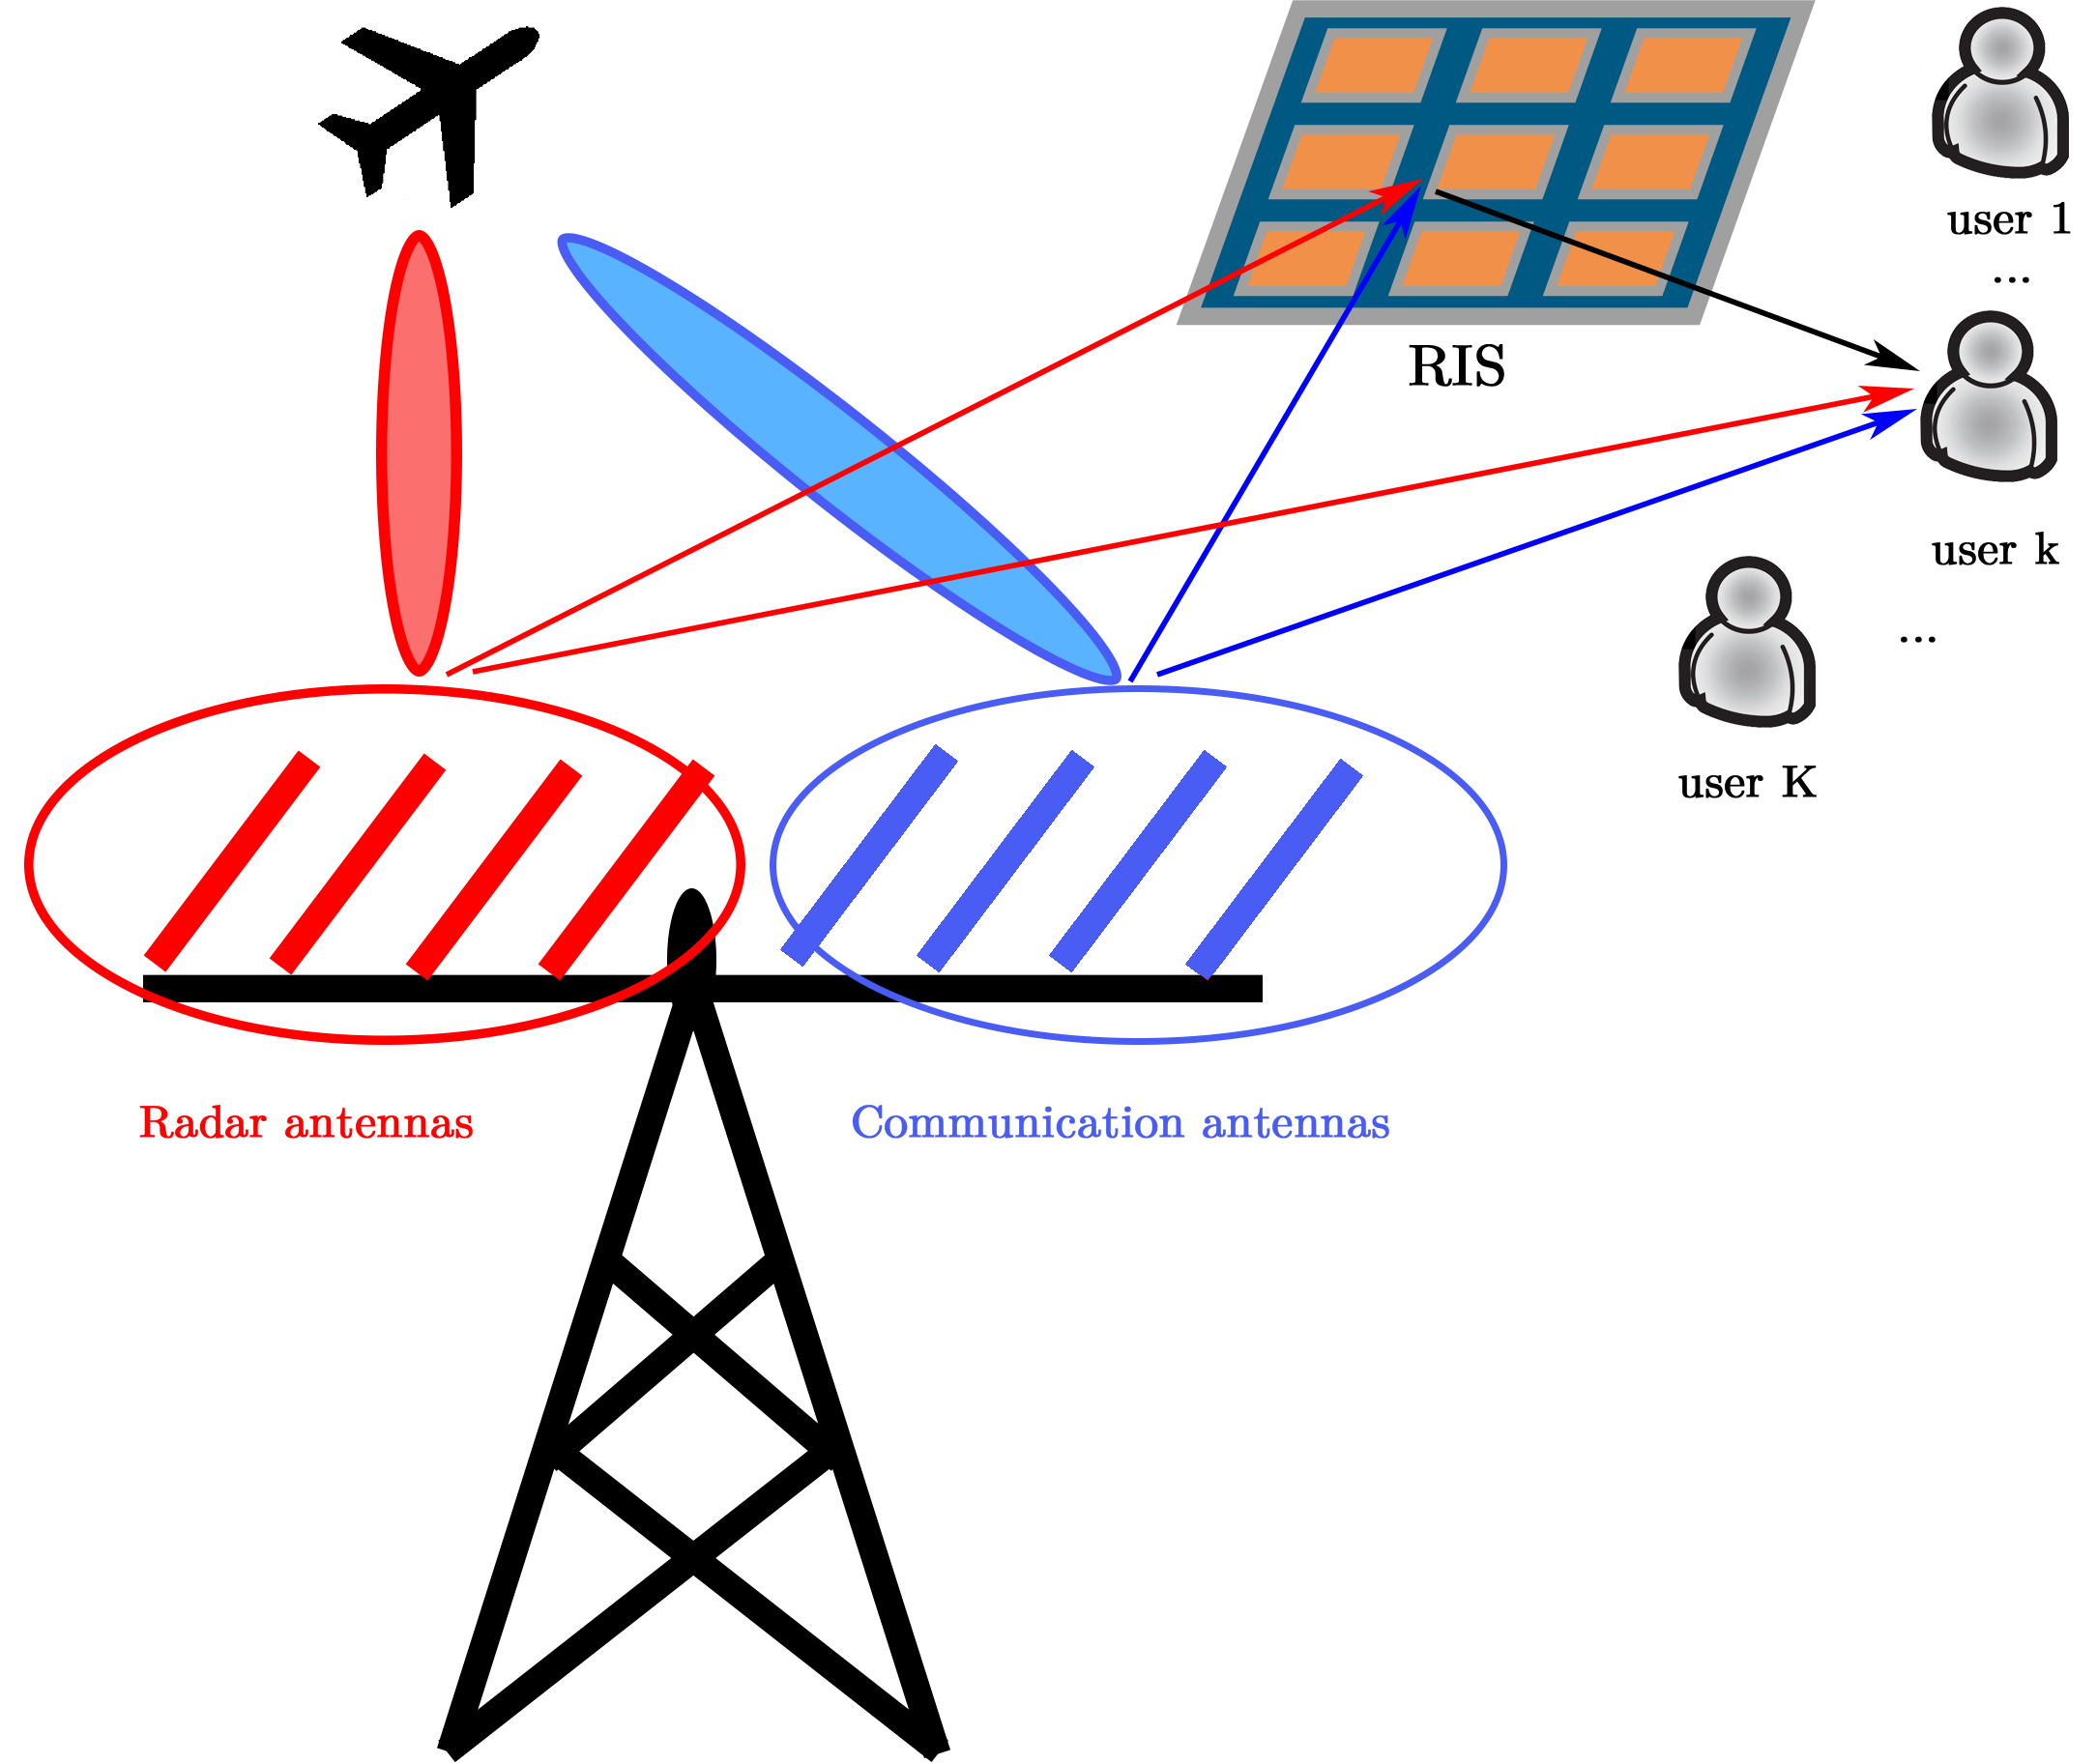
\includegraphics[width=0.4\linewidth]{./img/separated_setup.png}
        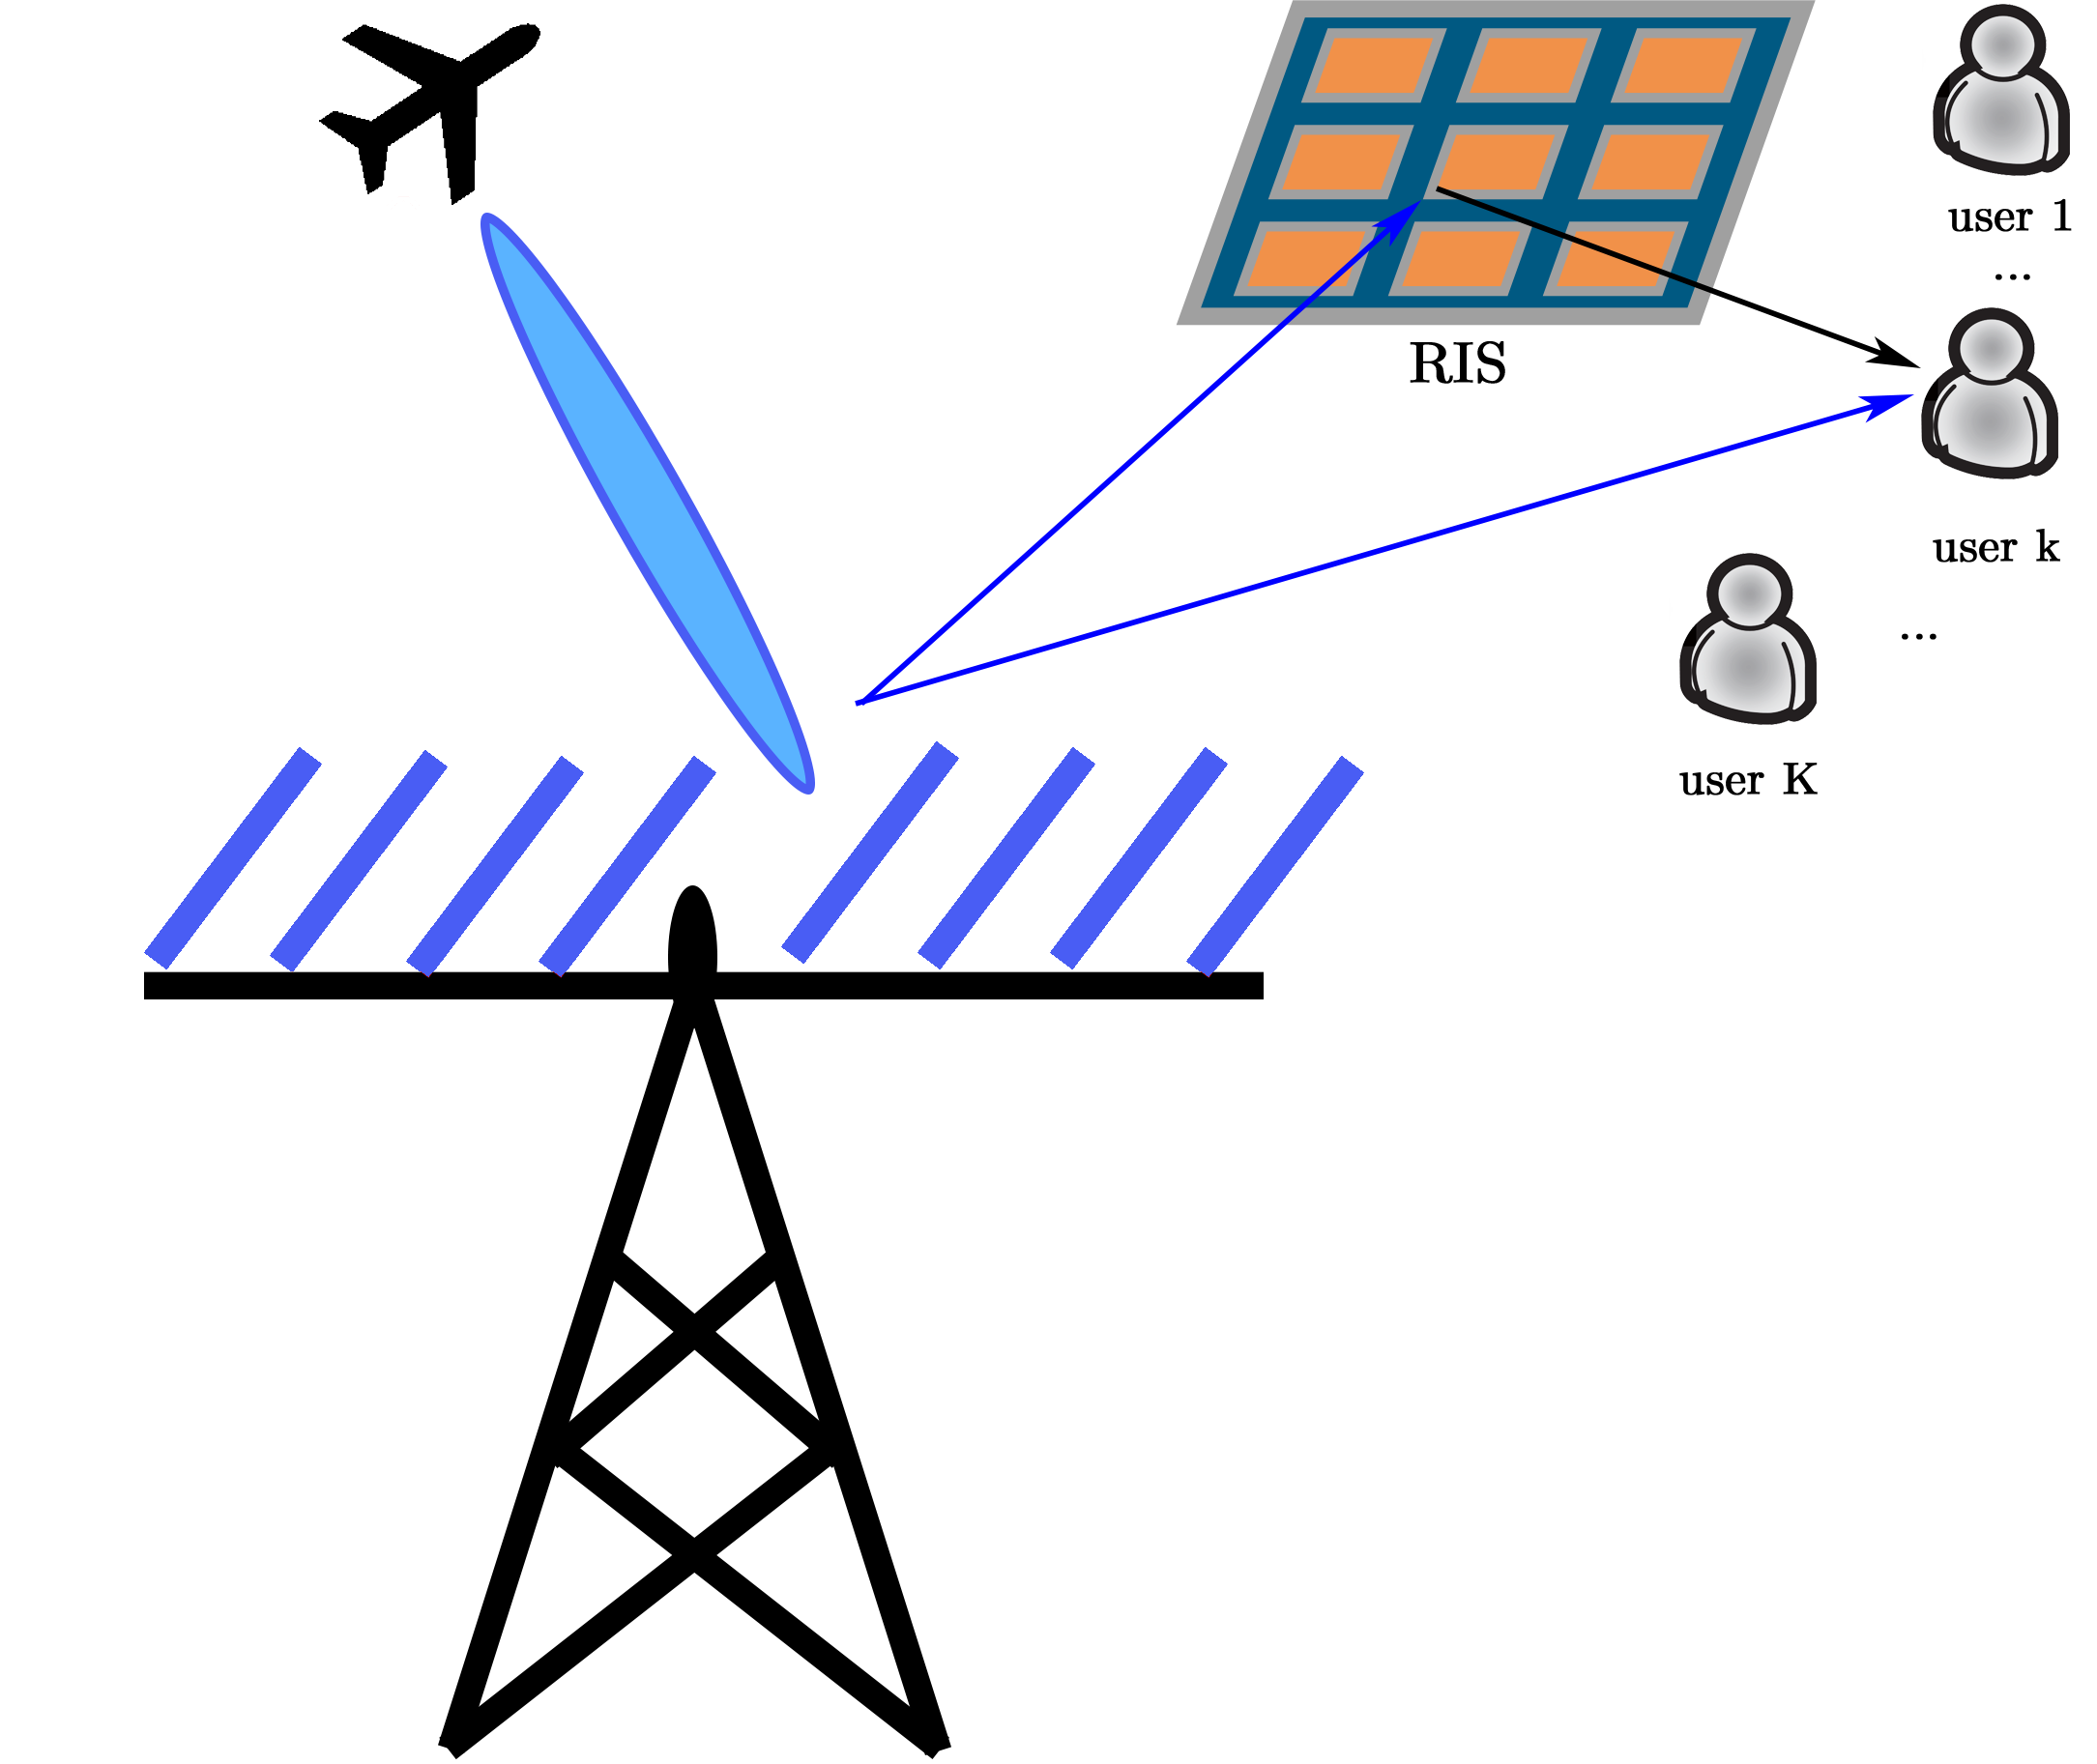
\includegraphics[width=0.4\linewidth]{./img/shared_setup.png}
    \end{figure}
\end{frame}

\begin{frame}
    \frametitle{RIS-aided Dual-Functional Radar and Communications Beamforming Design}

    \begin{block}{Why}
        \begin{itemize}
        \small
        \item To solve the spectrum congestion problem of radar and communication system;
        \item To investigate the benefit of RIS in DFRC system;
        \item Weighted Sum Rate (WSR) maximization has not been studied in RIS-aided DFRC system \cite{wang2020ris, jiang2021dfrc, wang2021joint}.
        \end{itemize}    
    \end{block}

    \begin{block}{How}
        \begin{itemize}
        \small
        \item Jointly design the active and passive beamforming to maximize the WSR and probing power;
        \item Apply a novel group or fully connected RIS model \cite{shen2020modeling};
        \item Simulate the system in both Rayleigh and Rician fading channels.
        \end{itemize}    
    \end{block}
\end{frame}

\begin{frame}
    \frametitle{RIS-aided Dual-Functional Radar and Communications Beamforming Design}
    \tiny
    \begin{figure}
        \centering
        \subfigure[Separated: Rayleigh channel]{
            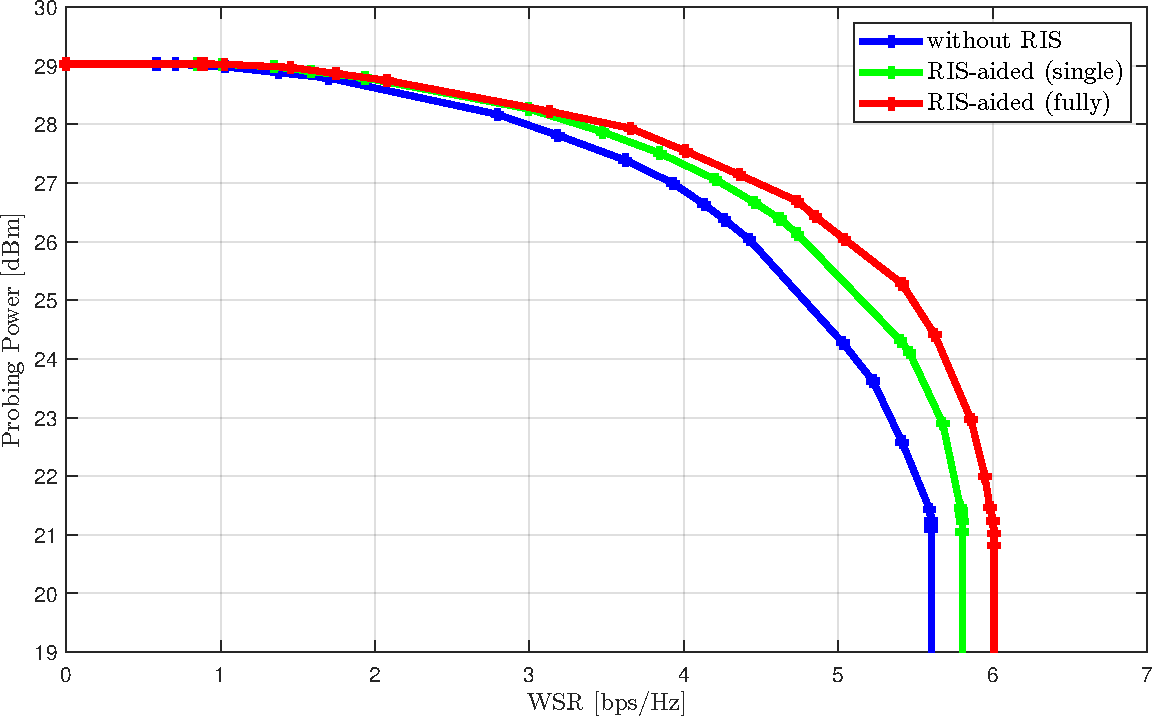
\includegraphics[width=0.4\linewidth]{./img/tradeoff_single_fully_a.pdf}
        }
        \subfigure[Separated: LOS channel]{
        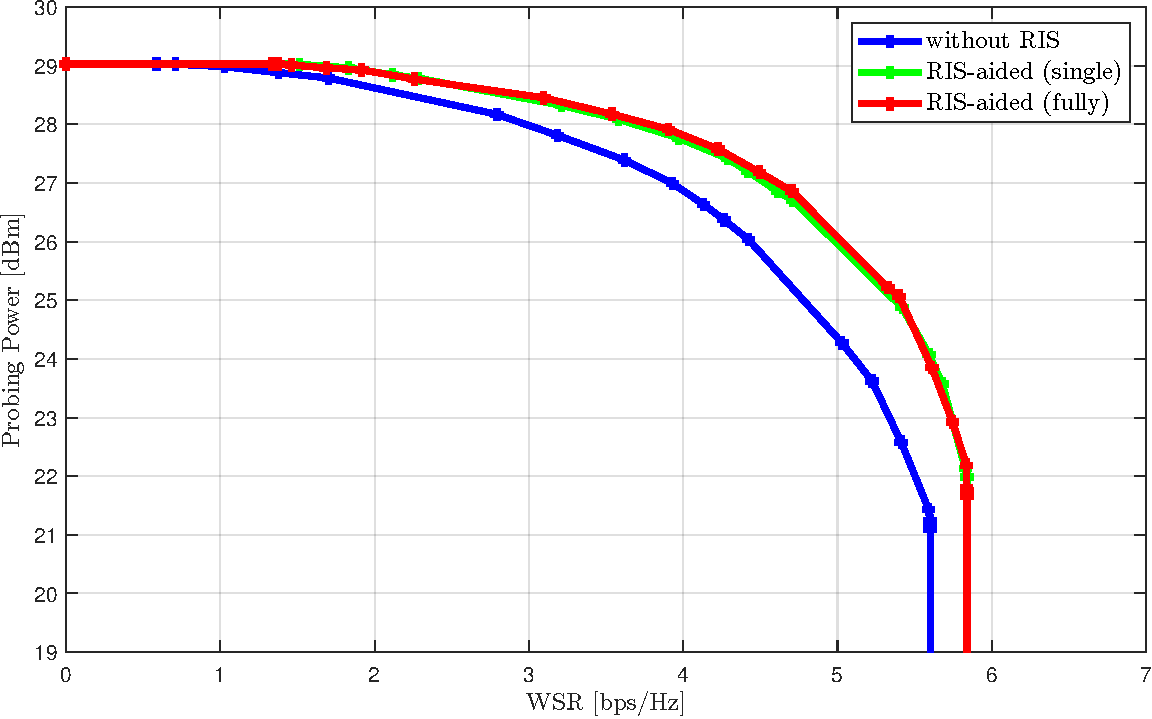
\includegraphics[width=0.4\linewidth]{./img/tradeoff_single_fully_b.pdf}
        }
        \subfigure[Shared: Rayleigh channel]{
            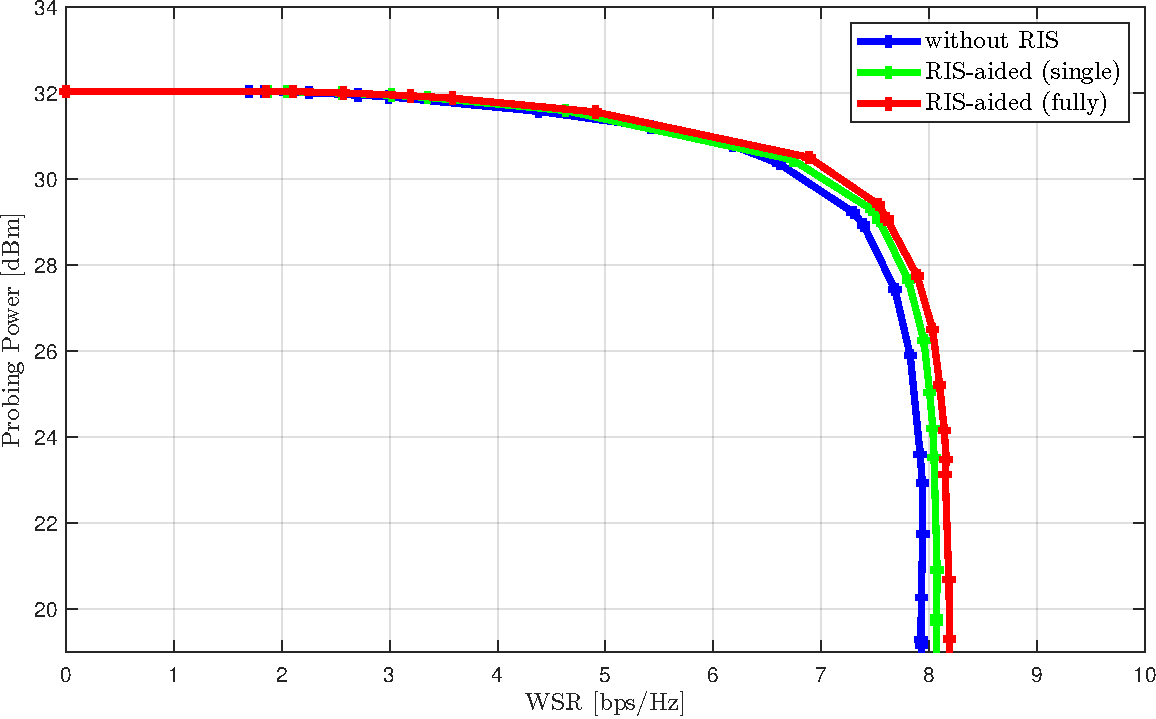
\includegraphics[width=0.4\linewidth]{./img/tradeoff_single_fully_c.pdf}
        }
        \subfigure[Shared: LOS channel]{
        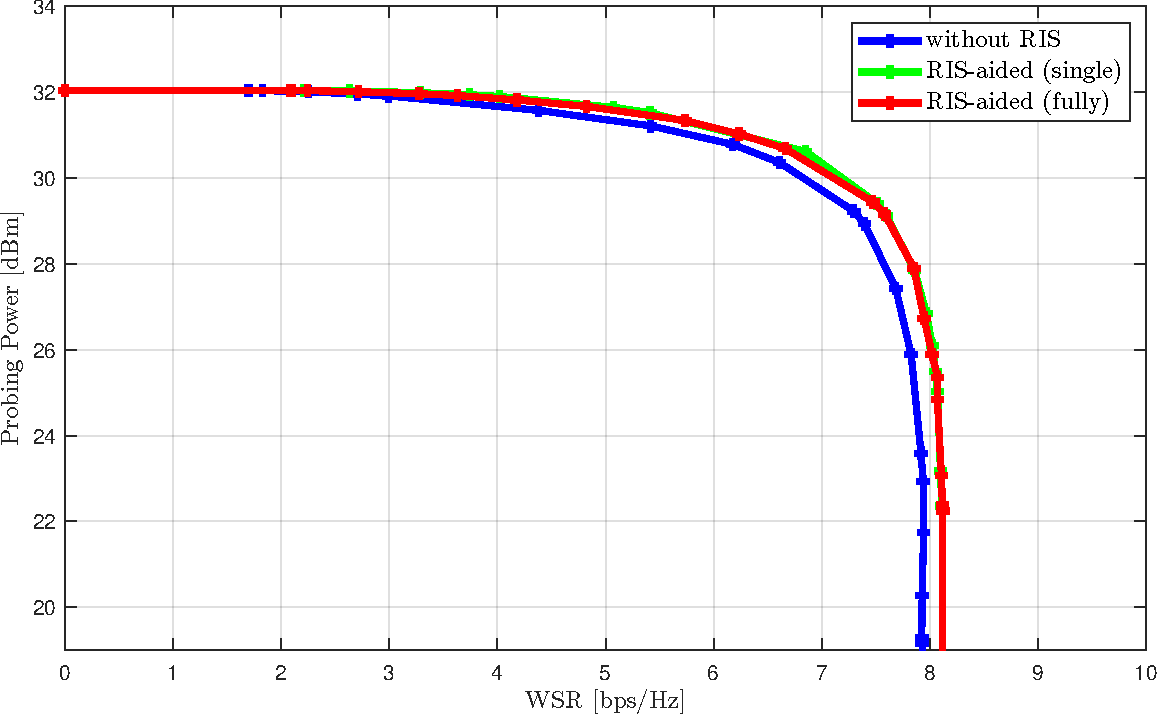
\includegraphics[width=0.4\linewidth]{./img/tradeoff_single_fully_d.pdf}
        }
    \end{figure}
\end{frame}

\begin{frame}
    \frametitle{RIS-aided Dual-Functional Radar and Communications Beamforming Design}
    \begin{figure}
        \centering
        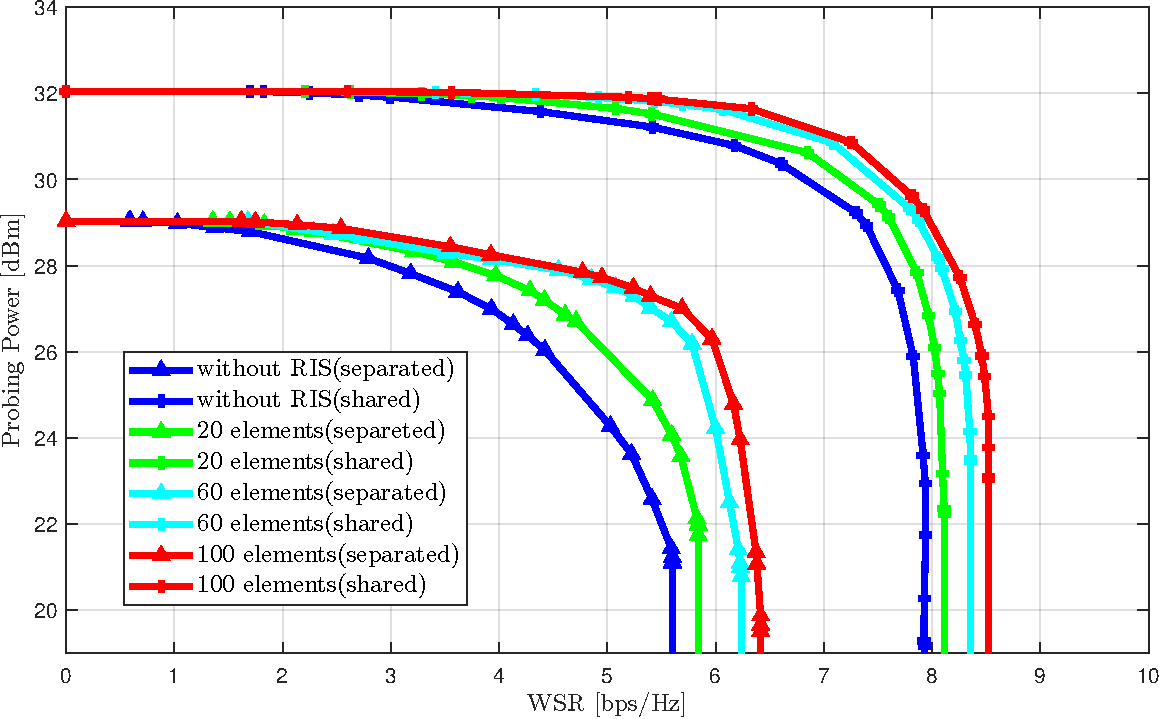
\includegraphics[width=0.7\linewidth]{./img/elements.pdf}
        \caption{Effect of the number of reflecting elements}
    \end{figure}
\end{frame}

\begin{frame}
    \frametitle{Estimate High-fidelity 3D Human Body Models from a Single Image using Deep Learning}
    \begin{block}{Conclusion}
        \begin{itemize}
        \small
        \item RIS is capable of enlarge the achievable region of WSR and probing power.
        \item The fully connected RIS is more powerful than the single connected in Rayleigh channel, but not in LOS channel.        
        \item More gain can be obtained by increasing the reflecting elements.
        \end{itemize}    
    \end{block}
    \begin{block}{Limitation}
        \begin{itemize}
        \small
        \item RIS is only used to improve the communication channel.
        \item The algorithm for the fully connected RIS converges slow. More efficient algorithm need to be found.
        \end{itemize}    
    \end{block}
\end{frame}
